\subsubsection{Plume in a 2D chunk}
\label{sec:plume-2d-chunk}
\textit{This section was contributed by Cedric Thieulot and Paul Bremner.}

This cookbook is inspired by Kellogg \& King (1997) \cite{keki97} but is not an attempt at reproducing the results of their publication. Their study was entirely carried out in dimensionless form. Here, however, we choose to build a similar experiment based on Earth dimensions and material properties.
Furthermore, in this cookbook we run strictly in 2D, whereas the original paper makes use of axisymmetry to restrict the problem to two velocity degrees of freedom \cite{kiha92}.

The two-dimensional domain is a section of an annulus, i.e. a 2D chunk with $ 3\pi/8 \leq \phi \leq \pi/2$. Free-slip boundary conditions are imposed on all boundaries. The inner and outer radii are $R\textsubscript{inner}=3480~\si{\km}$ and $R\textsubscript{outer}=6371~\si{\km}$, respectively.

Temperature boundary conditions are $T=T\textsubscript{surf}$ at the surface (outer boundary), insulating on the sides, and $T=T\textsubscript{cmb}$ at the inner boundary except along a patch $\phi > 7\pi/16$ where $T=T\textsubscript{patch}=T\textsubscript{surf}+\Delta T$.
Note that in the original publication the portion of the inner boundary that is not the patch is also insulating. By default, \aspect{} cannot accommodate two different boundary condition types on one boundary. So, we will prescribe plausible temperatures along the whole boundary, instead: $T\textsubscript{surf}=0\si{\celsius}$, $\Delta T=3000\si{\celsius}$, and $T\textsubscript{cmb}=2750\si{\celsius}$ (see for instance Steinberger \& Calderwood \cite{stca06}).

The domain contains a single fluid described by the `visco plastic' material model, with thermal expansion $\alpha=3\times 10^{-5}~\si{\per\kelvin}$, heat capacity $C_p=1250~\si{\joule\per\kg\per\kelvin}$, thermal diffusivity $\kappa=5.5\times 10^{-7}~\si{\square\meter\per\second}$ (corresponding to the thermal conductivity value  $k=\kappa \rho_0 C_p=2.25~\si{\watt\per\meter\per\kelvin}$), reference temperature $T_0=1023~\si{\kelvin}$, reference density  $\rho_0=3250~\si{\kg\per\cubic\meter}$, and viscosity $\eta_0=1.25\times 10^{23}$. Gravity is constant throughout the mantle with $g=9.81~\si{\meter\per\square\second}$.
With these parameters we find that the dimensionless Rayleigh number is 
\begin{equation}
Ra 
=\frac{\rho_0 g \alpha \Delta T (R\textsubscript{outer}-R\textsubscript{inner})^3}{\kappa \eta_0}
=10^6.
\end{equation}
In Kellogg \& King (1997), the dimensionless viscosity is temperature-dependent and defined as:
\[
\eta'(T')
=\eta_0' \exp\left[ \frac{E}{R \Delta T} \left( \frac{1}{T'+T_0'} -\frac{1}{1+T_0'}  \right)   \right],
\]
where $\eta_0'=1$ is the dimensionless viscosity, $E$ is the activation energy, and $R$ is the universal gas constant. The dimensionless temperature $T_0'$ is the surface temperature $T_{surf}$ divided by the temperature drop across the shell $\Delta T$. 
Assuming that the authors used the common relationship	 
\[
T'=\frac{T-T\textsubscript{surf}}{T\textsubscript{patch}-T\textsubscript{surf}}= \frac{T-T\textsubscript{surf}}{\Delta T}.
\]
then multiplying the equation above by $\eta_0$, it follows that:
\[
\eta(T)
=\eta_0 \exp\left[ \frac{E}{R} \left( \frac{1}{T-T\textsubscript{surf}  + T\textsubscript{surf}} 
-\frac{1}{T\textsubscript{patch}-T\textsubscript{surf} + T\textsubscript{surf}}  \right)   \right]
=\eta_0 \exp\left[ \frac{E}{R} \left( \frac{1}{T} -\frac{1}{T\textsubscript{patch}}\right) \right]
\]
so that $\eta(T_{patch})=\eta_0$.

Kellogg \& King (1997) investigated three cases:
$E/R \Delta T = \{0,0.25328,3\}$. Setting $R=8.31~\si{\joule\per\kelvin\per\mol}$ and $\Delta T=3000\si{\kelvin}$, the activation energy becomes $E=\{ 0, 6317.6 , 74829.6 \}\si{\joule\per\mole}$, lower than typical values (above 200~\si{kJ}, see for example Karato \& Wu \cite{KW93}).

The viscosity expression can be written as
\[
\eta(T)  
= \frac12 \underbrace{2 \eta_0  \exp\left( -\frac{E}{R T\textsubscript{patch}} \right) }_{A^{-1}} \exp \frac{E}{R T}  
\]
which is effectively a diffusion creep-type viscosity.
We find that $A^{-1} = \{ 2.5\times 10^{22}, 1.98\times 10^{22} , 1.6\times 10^{21} \}\si{\pascal\second}$, or  $A = \{ 4\times 10^{-24}, 5.05\times 10^{-24},  6.26\times 10^{-23}\} $. As in Kellogg \& King (1997) the viscosity is limited to  $\eta\textsubscript{max}=1000\eta_0$. 

We run the model to steady state for the reason given in Redmond \& King \cite{reki04} (which is similar to Kellogg \& King \cite{keki97}, only applied to Mars): ``We use steady state calculations so that we can separate time-dependent from parameter-dependent effects. Once again, it is unlikely that any Mars-sized, or larger, planetary body is in steady state. These calculations mainly serve as a guide, allowing us to determine the relationship between surface observations and internal parameters.''

Steady-state fields are shown in Fig.~\ref{fig:plume-diff-creep}. We find that the velocity fields are similar between the isoviscous and weakly temperature-dependent cases, where the convection cell occupies most of the domain. In contrast, the strongly temperature-dependent experiment showcases a large viscosity zone a few hundred kilometers thick (the thermal lithosphere), forcing the convection cell below it.i In other words, the thick lid insulates the convection cell, raising the temperature within it.

\begin{figure}
  \centering
  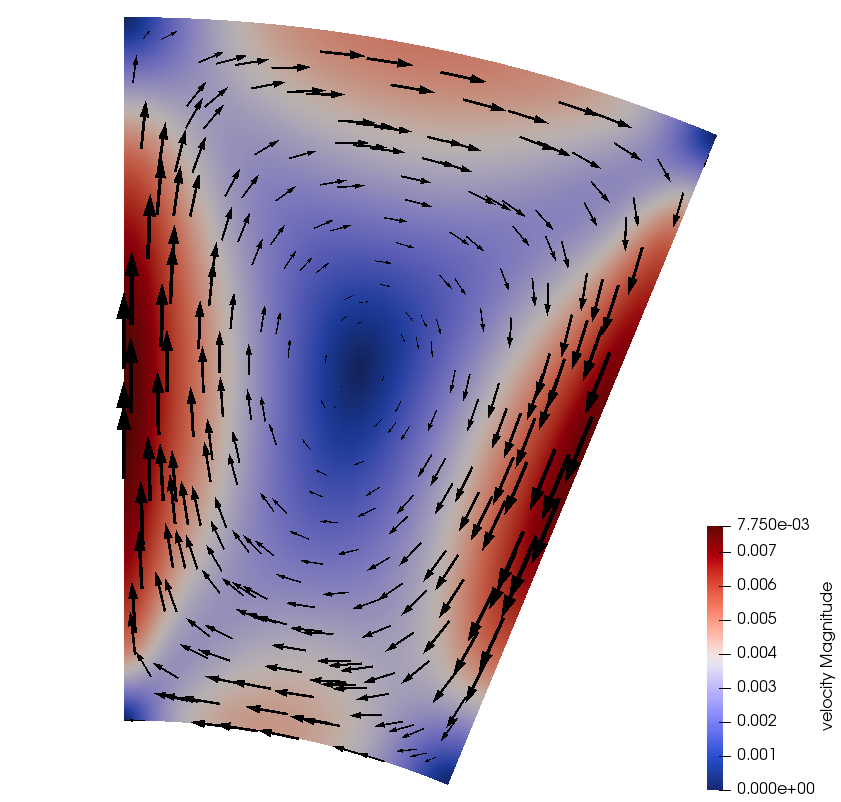
\includegraphics[width=5cm]{vel1}
  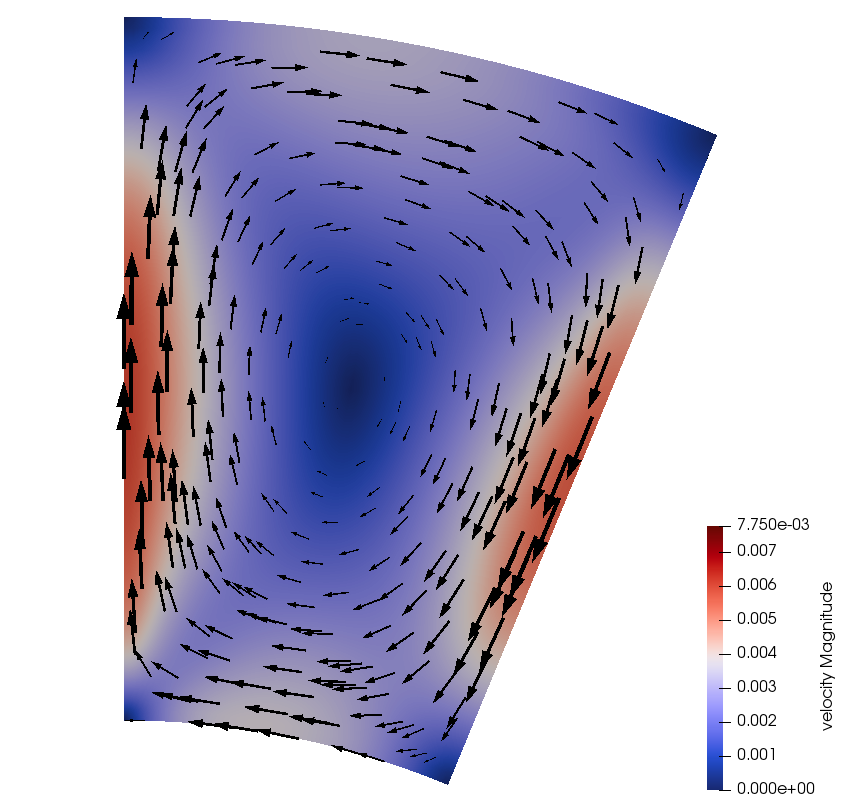
\includegraphics[width=5cm]{vel2}
  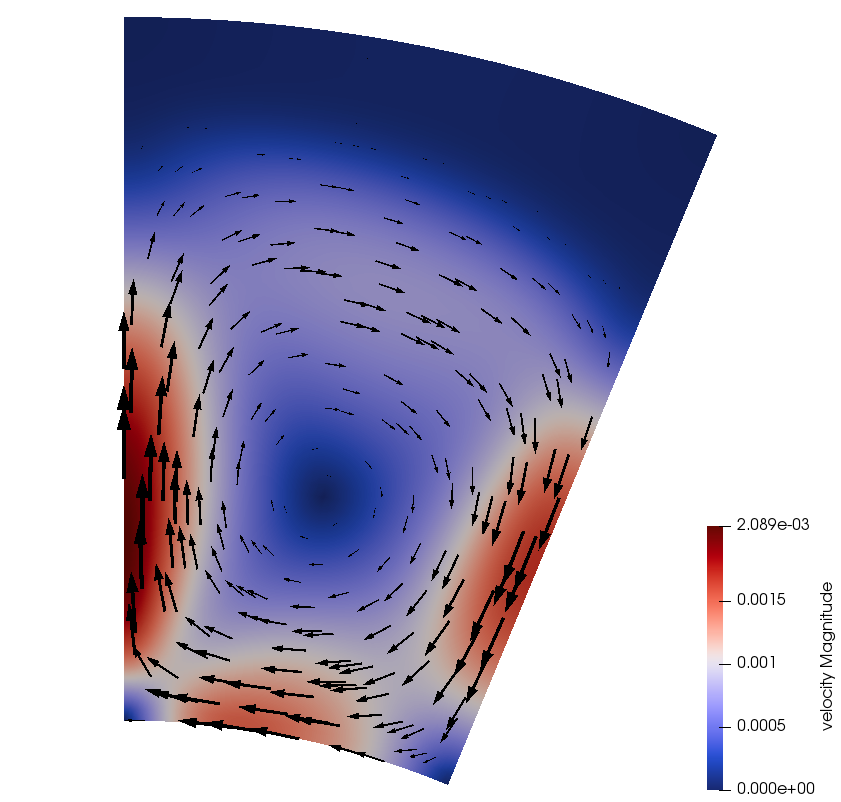
\includegraphics[width=5cm]{vel3}\\
  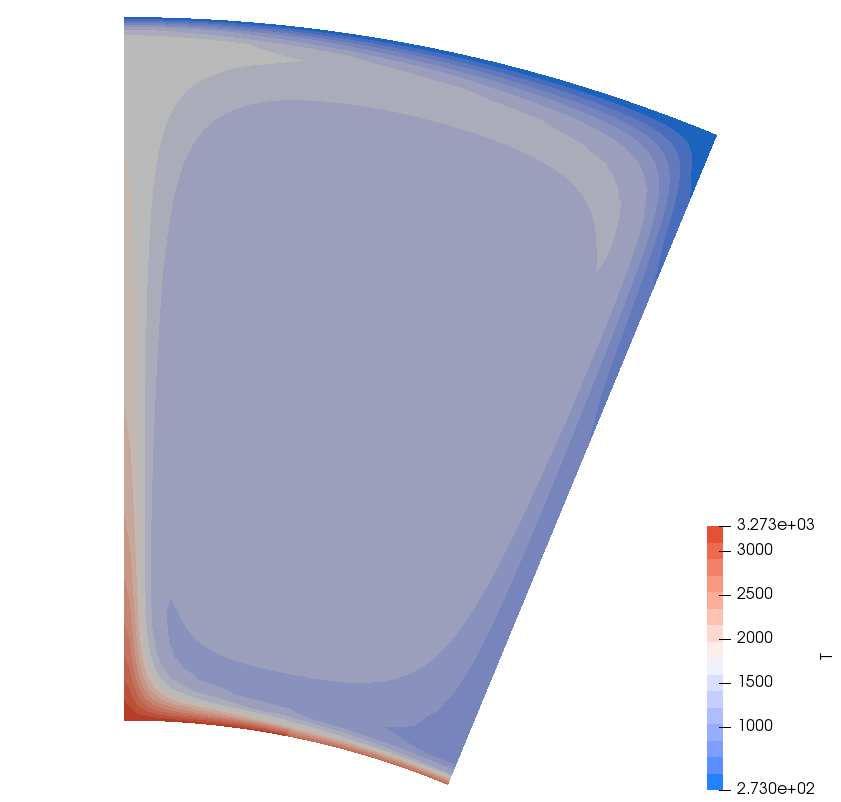
\includegraphics[width=5cm]{T1}
  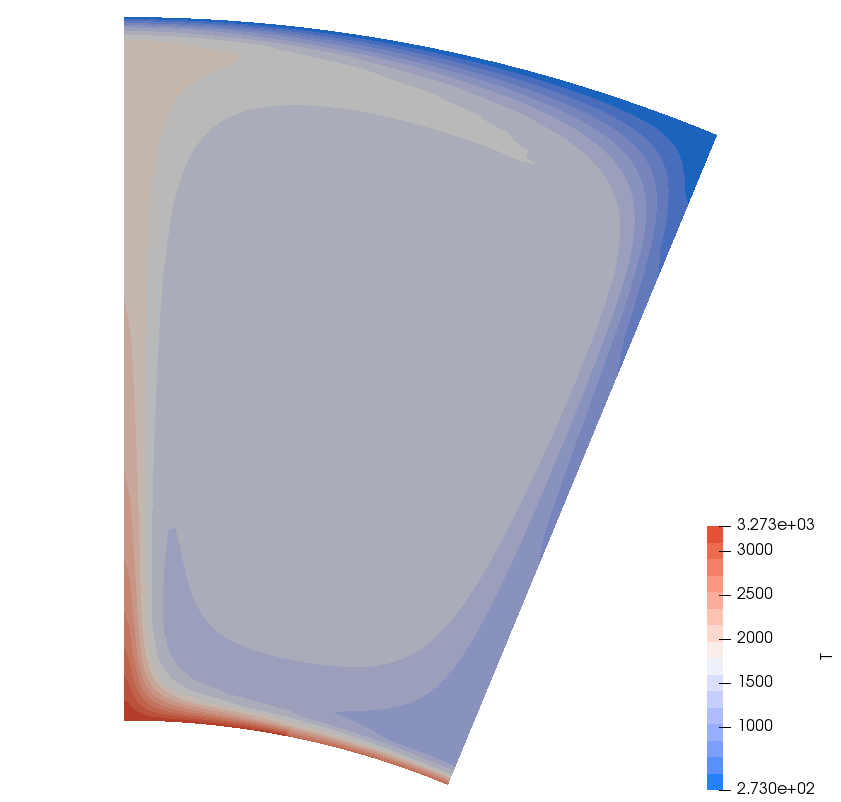
\includegraphics[width=5cm]{T2}
  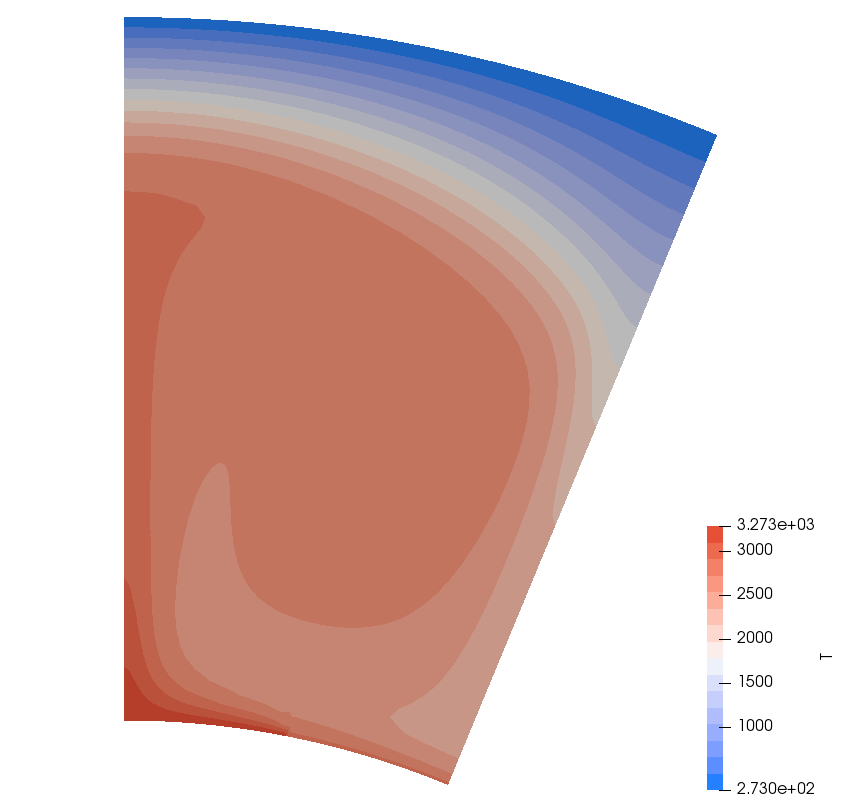
\includegraphics[width=5cm]{T3}\\
  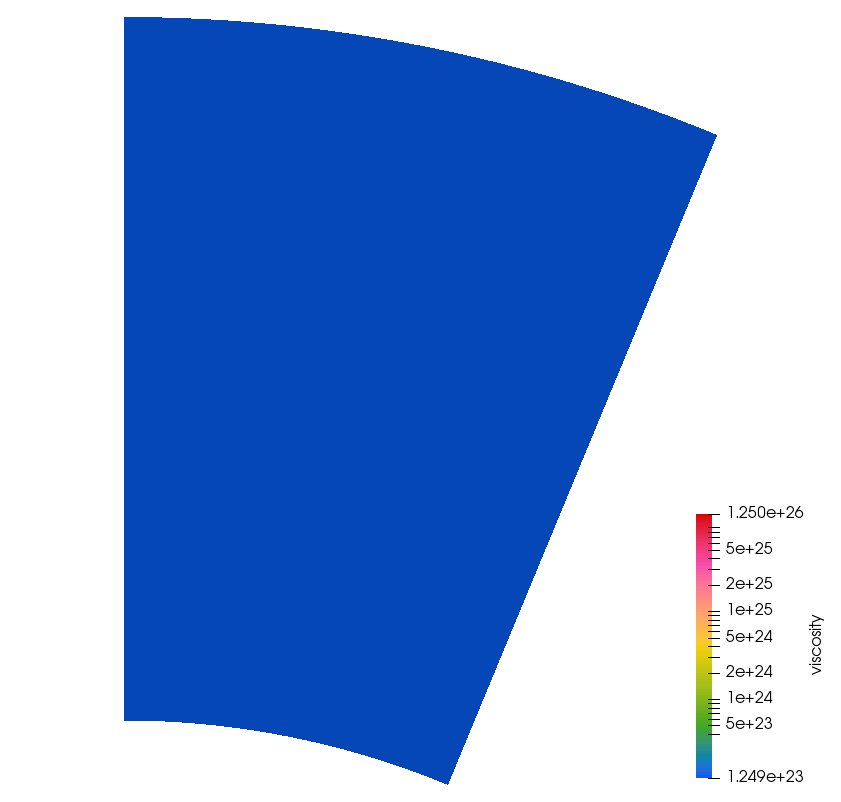
\includegraphics[width=5cm]{eta1}
  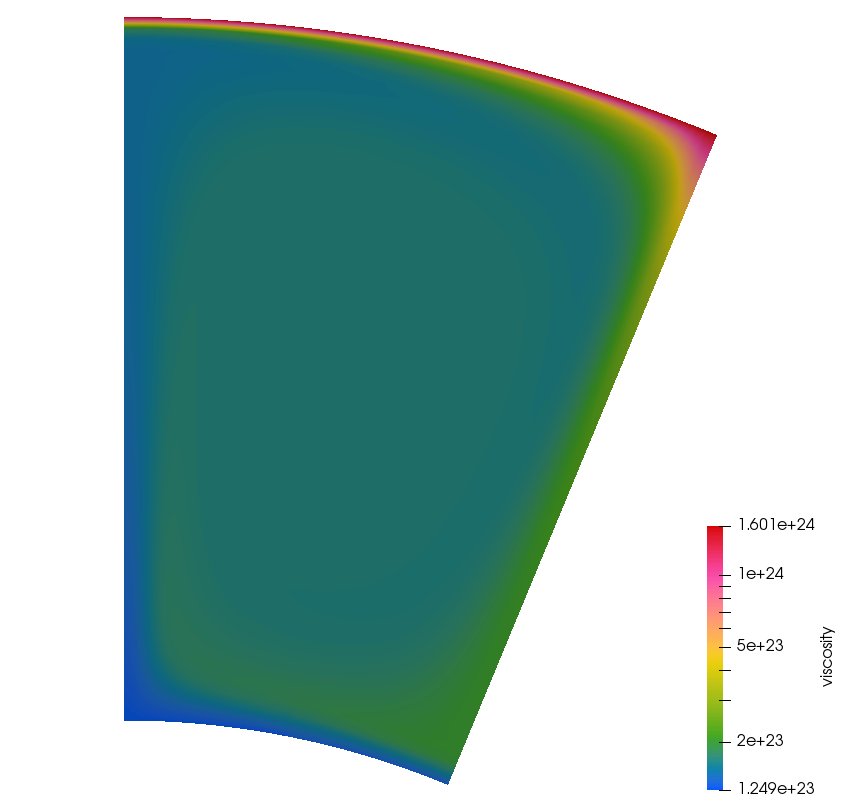
\includegraphics[width=5cm]{eta2}
  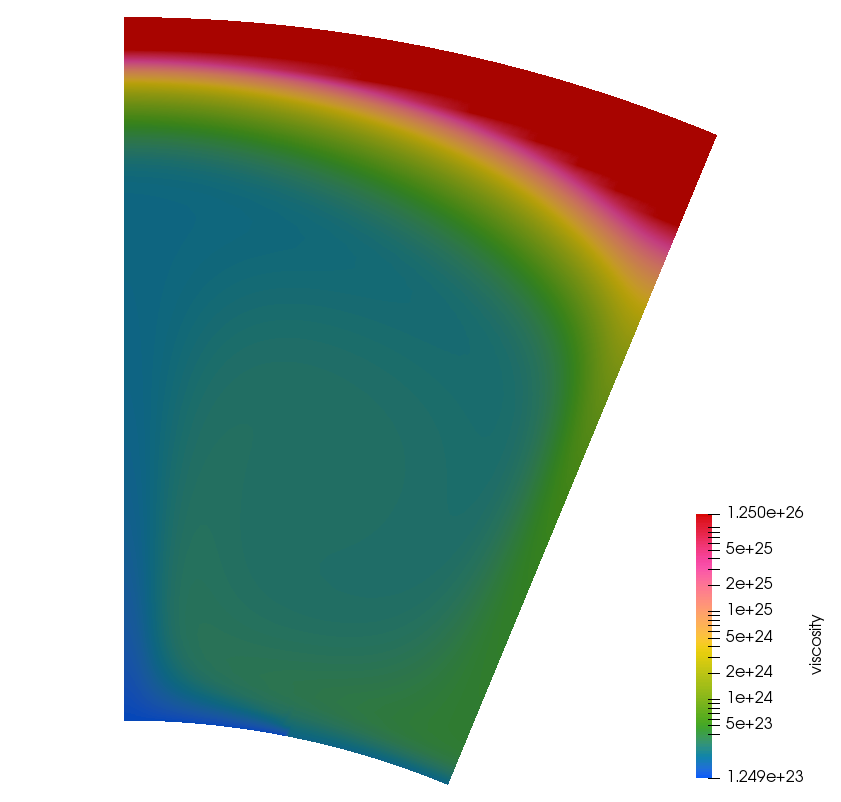
\includegraphics[width=5cm]{eta3}
  \caption{\it Plume in a 2D chunk. Columns from left to right: isoviscous case, weakly temperature dependent case, and strongly temperature-dependent case. Rows from top to bottom: Velocity, temperature, and viscosity field at steady state. Angular opening of $\pi/8$.}
  \label{fig:plume-diff-creep}
\end{figure}

Obtaining a steady state is contingent on the narrow angular opening. We find that simply increasing the angular opening from $\pi/8$ to $\pi/4$ yields only a statistical steady state, as multiple downwellings occur near the side but the system never stabilizes (see Fig.~\ref{fig:plume-angular-opening}). Also, decreasing $\eta_0$ by a factor 10 would yield $Ra=10^7$. In this case, too, a statistical steady state is reached (not shown here).

\begin{figure}
  \centering
  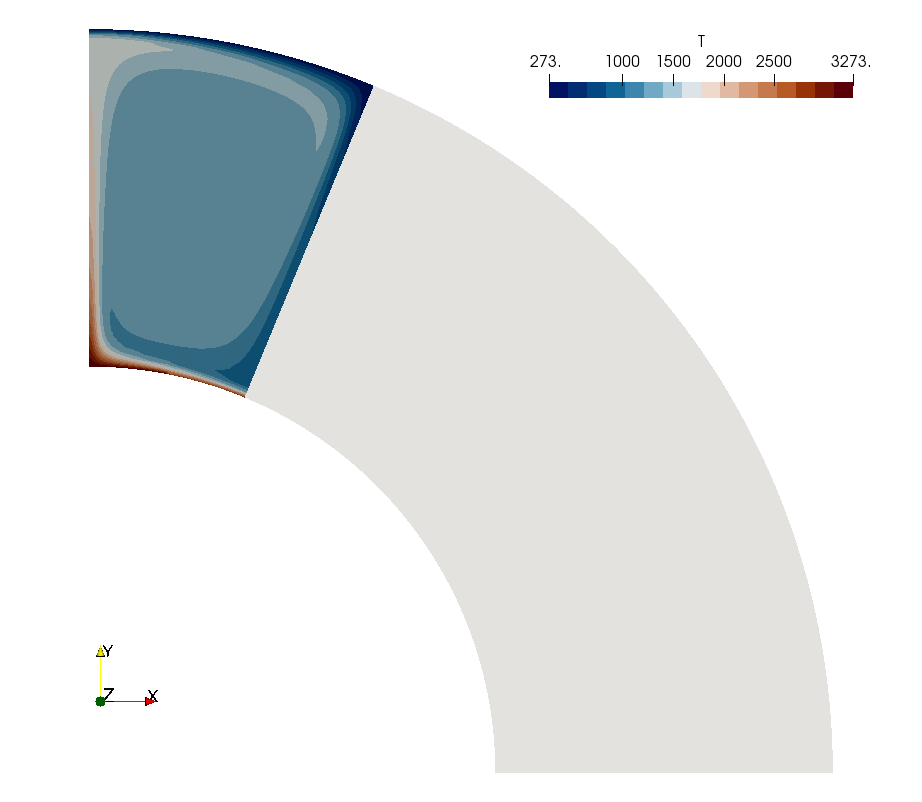
\includegraphics[width=5cm]{exp1_22}
  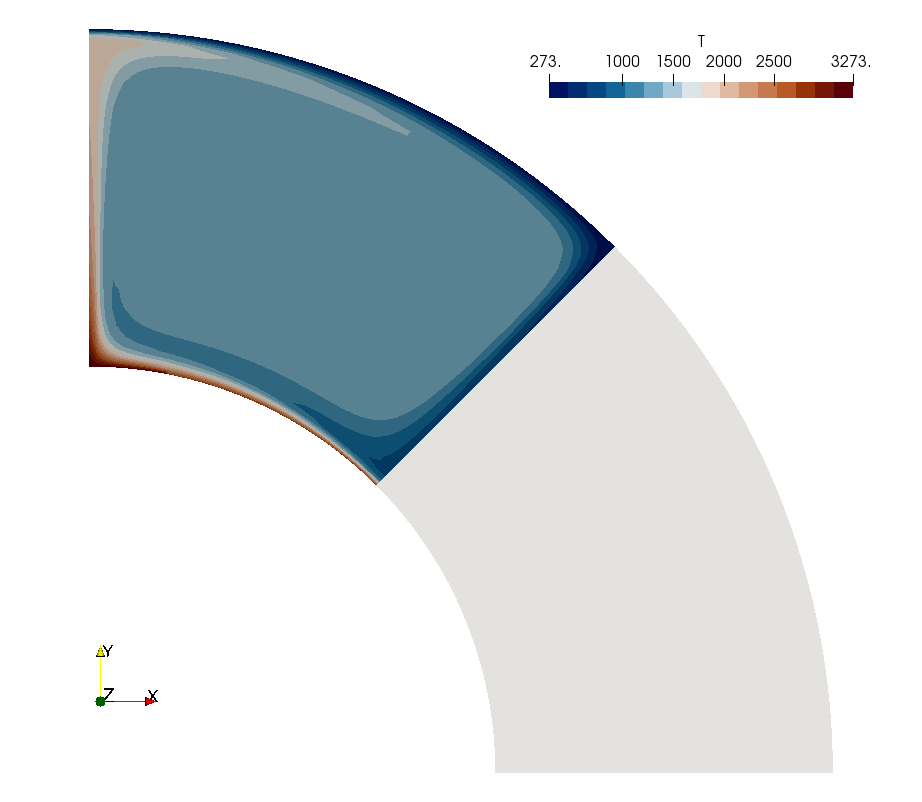
\includegraphics[width=5cm]{exp1_45}
  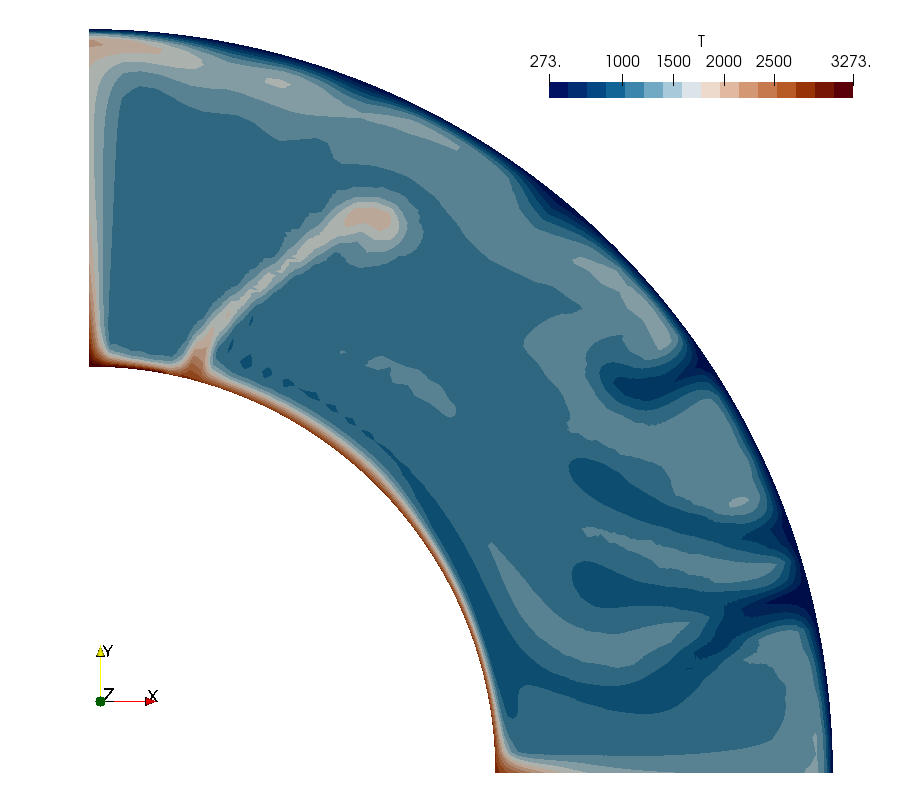
\includegraphics[width=5cm]{exp1_90}
  \caption{\it Plume in a 2D chunk: Temperature at the end of the run. From left to right: Angular opening of
$\pi/8$, $\pi/4$ and $\pi/2$. The first two have reached a steady state while the third one has not.}
  \label{fig:plume-angular-opening}
\end{figure}

Fig.~\ref{fig:plume-diff-creep-vrms} shows the time evolution of the root mean square velocity as a function of time. 
As mentioned above, no active planet is at steady state so the time on the horizontal axis is not really meaningful. Also, it is easy to show that the path to steady state (if at all attained) is vastly influenced by the initial temperature field.
We find that the average velocities are smaller in the models with larger activation energy, which is reasonable since on average viscosities increase with an increase in activation energy $E$. Also, although it looks like the system reaches steady state for the $\pi/2$ opening angle it ultimately proves unstable and becomes chaotic, akin to the figure on the cover of this manual. Please check the corresponding video \url{https://youtu.be/FN2BBmbiA8E} to see the system for the entire duration of the simulation.

\begin{figure}
  \centering
  \includesvg[width=10cm]{vrms.svg}
  \caption{\it Plume in a 2D chunk: Root mean square velocity for each experiment.}
  \label{fig:plume-diff-creep-vrms}
\end{figure}

